\begin{frame}{Teoretyczne podstawy SMT}
	\begin{figure}[htbp]
		\centering
		\begin{minipage}{\textheight}
			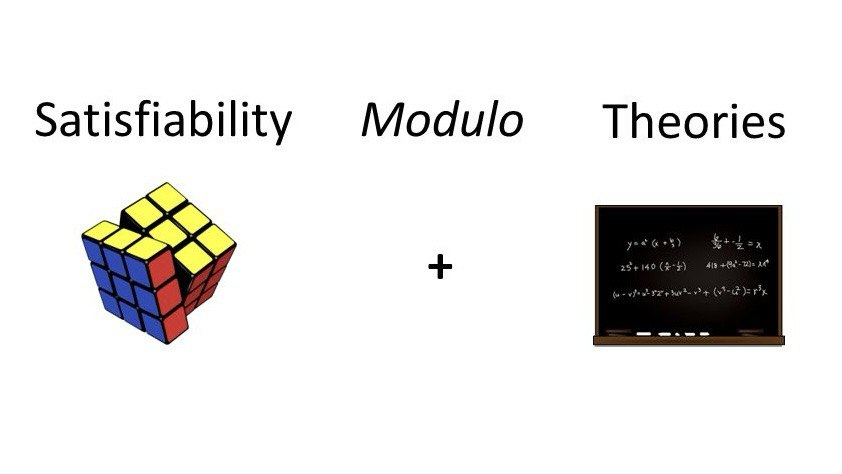
\includegraphics[width=\textheight]{./slides/smt.jpg}
		\end{minipage}
	\end{figure}
    \begin{itemize}
    	\item SMT łączy problem spełnialności logicznej z różnymi teoriami matematycznymi.
    	\item Zadaniem jest stwierdzenie, czy istnieją wartości zmiennych spełniające zarówno ograniczenia logiczne, jak i dodatkowe z teorii matematycznej.
    \end{itemize}
\end{frame}